\section{تحریک مغز}

تحریک مغز می تواند به روش های مختلف انجام شود که در دو دسته کلی تهاجمی و غیرتهاجمی جای می‌گیرند. تحریک مغناطیسی فراجمجمه‌ای 
\LTRfootnote{Transcranial Magnetic Stimulation (TMS)}
و تحریک الکتریکی جریان مستقیم فراجمجمه‌ای
\LTRfootnote{Transcranial Direct Current Stimulation (tDCS)}
که کاربرد بیشتری نسبت به سایر روش‌ها دارند، از جمله روش‌های غیرتهاجمی تحریک مغز به شمار می‌روند.
برخی از اشکال مختلف تحریک غیرتهاجمی مغز را می‌توانید در شکل 
\ref{fig:nibs}
ببینید.

\begin{figure}
     \centering
     \begin{subfigure}[t]{0.7\textwidth}
         \centering
         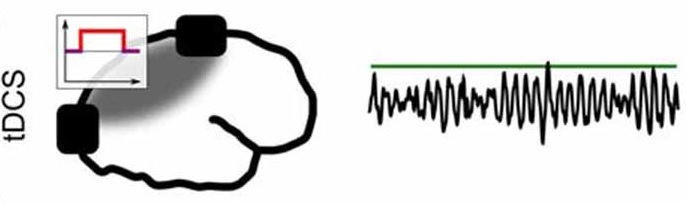
\includegraphics[width=\textwidth]{tdcs}
         \caption{تحریک الکتریکی فرا جمجمه‌ای با جریان مستقیم }
         \label{fig:tdcs}
     \end{subfigure}
     \\
     %\hfill
     \begin{subfigure}[t]{0.7\textwidth}
         \centering
         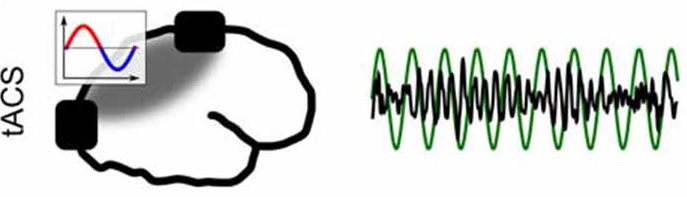
\includegraphics[width=\textwidth]{tacs}
         \caption{    تحریک الکتریکی فرا جمجمه‌ای با جریان متناوب }
         \label{fig:tacs}
     \end{subfigure}
     \\
  %   \hfill
     \begin{subfigure}[t]{0.7\textwidth}
         \centering
         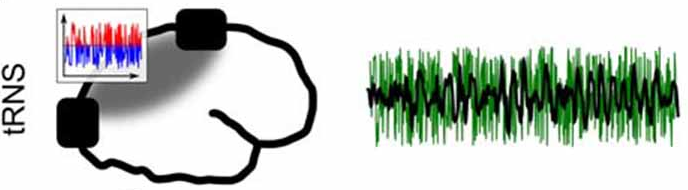
\includegraphics[width=\textwidth]{trns}
         \caption{    تحریک الکتریکی فرا جمجمه‌ای با جریان نویز تصادفی}
         \label{fig:trns}
     \end{subfigure}
     \\
         \begin{subfigure}[t]{0.7\textwidth}
         \centering
         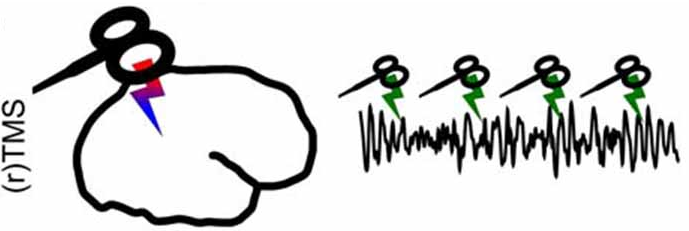
\includegraphics[width=\textwidth]{tms}
         \caption{تحریک مغناطیسی مغز}
         \label{fig:tms}
     \end{subfigure}
        \caption{اشکال مختلف تحریک غیرتهاجمی مغز. تصویر سمت چپ طرحی از نحوه اعمال تحریک و ولتاژ بین الکترودها را با گذشت زمان نشان می دهند. مناطق خاکستری توزیع میدان الکتریکی  در منطقه هدف را نشان می‌دهد. تصویر سمت راست نشان دهنده سیگنال تحریک (سبز) نسبت به  \lr{ EEG }(سیاه) از یک منطقه هدف بالقوه است.
         }
        \label{fig:nibs}
\end{figure}

تحریک مغزی فراجمجمه‌ای و تحریک مغزی عمیق برای درمان طیف وسیعی از بیماری‌های سیستم عصبی و ناهنجاری‌های شناختی از پارکینسون و صرع تا افسردگی، اضطراب و اعتیاد استفاده شده و کارآیی آن مشاهده شده است. با وجود این سازوکار تاثیر تحریک مغزی و علت کارایی آن تقریبا ناشناخته است و عمدتا پروتکل‌های موجود با روش سعی و خطا بوجود آمده و توسعه یافته‌اند. شناخت سازوکار این تاثیرات بر روی دینامیک شبکه‌های عصبی و به طور خاص بر نوسانات جمعی سلول‌های عصبی، برای توسعه هدفمند استفاده از آن‌ها بسیار اساسی است. 


زمینه تحریک غیر تهاجمی مغز در 30 سال گذشته و به ویژه در 15 سال گذشته به طور قابل توجهی توسعه یافته است. مقاله اصلی از بارکر و همکاران 
\cite{barker1985non}
نشان داد كه می‌توان جریان تحریكی را به روش نسبتاً بدون درد با استفاده از تحریک مغناطیسی فرا جمجمه‌ای
 (\lr{TMS}) 
به سیستم عصبی مركزی اعمال کرد. این اتفاق انگیزه فراوانی برای توسعه در این زمینه ایجاد کرده بود. پس از این گزارش مهم، دانشمندان و پزشکان دوباره شروع به بررسی تأثیر بالینی تحریک غیرتهاجمی مغز در ابتدا به عنوان یک روش تشخیصی و سپس به عنوان یک ابزار بالینی کردند.
جالب اینجاست که استفاده از
 \lr{TMS}
به عنوان یک روش تشخیصی آن‌طور که پیش‌بینی می‌شد توسعه نیافت. در پژوهش‌های مختلف نشان داده شده است که
 \lr{TMS}
نقش محدودی به عنوان نشانگر تشخیص بیماری‌های مرتبط با دستگاه عصبی مانند بیماری پارکینسون دارد. با این حال، 
\lr{TMS}
 یا شکل تکراری آن، 
\lr{rTMS}
، با اثرات بالینی قابل توجهی در شرایط اعصاب و روان همراه است
\cite{rossi2009safety}
. در سال 2009 ، این روش توسط سازمان غذا و داروی آمریکا 
\LTRfootnote{US Food and Drug Administration (FDA)}
 به عنوان درمانی برای افسردگی مقاوم 
\LTRfootnote{Refractory depression}
تأیید شد.
پس از علاقه شدید اولیه به 
\lr{TMS}
، دانشمندان این حوزه شروع به بررسی این موضوع کردند که آیا جریان‌های زیاد (مانند جریانهای القا شده توسط 
\lr{TMS}
) برای القای تغییر در شکل‌پذیری عصبی مورد نیاز هستند. این سوال باعث شد دو گروه، یكی در گوتینگن (آلمان) و دیگری در میلان (ایتالیا) به جستجوی یك روش قدیمی تحریک غیرتهاجمی مغز، تحریک جریان مستقیم فراجمجمه‌ای 
\lr{(tDCS)}
بپردازند
\cite{nitsche2008transcranial}.
مطالعات اولیه از این گروه‌ها نشان داد که با توجه به ثابت بودن جهت جریان‌، جریان‌های الکتریکی ضعیف نیز می‌توانند تغییرات قابل توجهی در تحریک‌پذیری قشر ایجاد کنند. این نتایج راه جدیدی را برای کشف مدولاسیون عصبی با جریان های الکتریکی ضعیف باز کرد. در استفاده‌های درمانی برای تقویت اثرات تحریک مغز از ترکیبی از تکنیک‌های مختلف تحریک غیر تهاجمی مغز استفاده می‌شود. با همه این اوصاف، صرف نظر از تعداد قابل توجه مطالعات انجام شده در مورد تحریک غیر تهاجمی مغز، هنوز این پرسش وجود دارد که آیا تاثیر بالینی این روش‌ها معنی دار است؟
%\footnote{معنی دار است یعنی چی؟ از نظر آماری یا از نظر علت و معلولی؟}


تحریک الکتریکی روی یک فیبر عصبی می تواند باعث تولید پتانسیل عمل شود. در این حالت، ولتاژ و یا جریان تحریک باید از آستانه ولتاژ تحریک غشای سلول، بزرگ تر باشد (تحریک بالای آستانه‌ای). یک رویکرد دیگر آن است که ولتاژ غشا سلول عصبی به گونه ای تغییر داده شود که بدون بوجود آمدن پتانسیل عمل، آستانه تحریک‌شوندگی تغییر کند (تحریک زیر آستانه‌ای) که به این وسیله امکان افزایش یا کاهش تحریک‌پذیری سلول فراهم می‌شود.

تحریک الکتریکی جریان مستقیم فراجمجمه‌ای، یک تحریک غیرتهاجمی و زیر آستانه‌ای با هدف ایجاد شرایط مناسب برای تغییر تحریک پذیری عصبی است که در آن معمولاً از دو الکترود صفحه‌ای بزرگ (95-65 سانتی متر مربع) و جریان تقریبا 9 میلی آمپر استفاده می شود. از این روش به عنوان یک راه حل درمانی برای درمان مشکلات عصب شناختی (مانند پارکینسون، سکته مغزی و آلزایمر) و مشکلات روان پزشکی (مانند افسردگی، اختلالات خواب و زوال عقل) استفاده می شود. علاوه بر این، تحقیقات نشان داده است که این روش می تواند موجب ارتقای عملکردهای شناختی مغز مانند توجه، تصمیم گیری، یادگیری، حافظه و شکل‌پذیری سیناپسی در انسان و حیوان شود.

شناخت ساز و کار اثرگذاری انواع مختلف تحریک‌های مغز از این لحاظ حائز اهمیت است که به طراحی پروتکل و سیستم مناسب جهت دست‌یابی به اثر مطلوب از تحریک مغز کمک می‌کند. رویکرد مدل‌سازی که در بسیاری از تحقیقات از آن استفاده شده است می‌تواند در شناخت این ساز و کار موثر باشد. مدل‌سازی فیزیولوژیکی با تجمیع شواهد نوروفیزیولوژیک مختلف قادر به شبیه‌سازی عملکرد نورون‌ها تحت شرایط مورد نظر بوده و به این طریق، شکاف بین کارکرد مشاهده شده از فعالیت عصبی و شواهد آزمایشگاهی که به دلایل فنی (برای مثال دشوار بودن ثبت در سطوح و مقیاس های زمانی مختلف) محدود شده‌اند را برطرف می‌کند. 


\subsection{تحریک عمیق مغز}

%از کتاب پیتر تاس:
%\\
مغز از انبوهی از خوشه‌های نورونی تشکیل شده است که به طرز پیچیده‌ای به هم متصل شده‌اند. این خوشه‌هابا استفاده از اتصالات ساختاری دو طرفه یا یک طرفه، گروه‌ها یا حلقه‌هایی را تشکیل می‌دهند. 

در برخی از اختلالات عصبی به عنوان مثال در بیماری پارکینسون، درون حلقه‌های خاصی خوشه‌های نورونی فعالیت ریتمیک غیرعادی و ناهنجار دارند. برای درمان چنین بیماری‌هایی، الکترودهایی با دقت میلی‌متر درون مغز، درون یک خوشه عصبی خاص کاشته می‌شوند. این الکترودها برای سرکوب و تضعیف فعالیت نورونی پاتولوژیک بوسیله تحریک با فرکانس بالا استفاده می‌شوند. چنین درمانی امروزه برای بیمارانی که از بیماری پارکینسون پیشرفته رنج می‌برند و دیگر از درمان های دارویی نفعی نمی‌برند استفاده می‌شود. 

تاکنون مشخص نیست که چگونه این نوع تحریک فعالیت نورونی ریتمیک که باعث ایجاد لرزش در بیماران پارکینسونی می‌شود را سرکوب می‌کند. بر این اساس درک صحیح نظری از رفتار دینامیکی خوشه های نورونی ناشی از تحریک می‌تواند به بهبود تکنیک‌های تحریک کمک کند.

تحریک عمقی مغز
\LTRfootnote{Deep brain Stimulation (DBS)}
 نوعی روش درمانی (جراحی) در پزشکی است که در طی آن الکترودهایی در داخل مغز بیمار قرار داده می‌شوند. این الکترودها پس از کاشته شدن در مغز به یک دستگاه مولد پالس الکتریکی
 \LTRfootnote{Pulse Generator}
  متصل می‌شوند. پالس الکتریکی تولید شده توسط دستگاه پالس ژنراتور از طریق الکترودهای کاشته شده در مغز به بافت‌های عمقی مغز انتقال یافته و از این طریق اثر درمانی خود را اعمال می‌نماید. روش درمانی تحریک عمقی مغز برای اولین بار در انسان در سال ۱۹۸۷ توسط جراح مغز و اعصاب فرانسوی علیم-لویی بن عبید
\LTRfootnote{Alim-Louis Benabid}
به کار گرفته شد. سیستم تحریک عمقی مغز سه بخش دارد که درون بدن نصب می شوند:
\begin{itemize}
\item تحریک‌کننده عصبی: دستگاهی ضربان ساز و قابل برنامه ریزی است که با باتری کار میکند و باعث تولید پالس های الکتریکی می‌شود. این دستگاه زیر پوست قفسه سینه یا شکم قرار می‌گیرد (شکل 
\ref{fig:dbs00}
).
\item سیم های انتقال جریان: سیم هادی که لیدها را به تحریک‌کننده متصل می‌کنند. این سیم معمولاً در زیر پوست جایگذاری می‌شود و از جمجمه به پشت گوش و گردن و نهایتا به سینه می‌رسد (شکل 
\ref{fig:dbs00}
).
\item لید: یک سیم با تعدادی الکترود در نوک آن است که پالس های الکتریکی را به بافت مغزی منتقل می کند. الکترود ها درون مغز قرار میگیرند و از یک سوراخ کوچک در جمجمه به سیم ها متصل شده اند (شکل 
\ref{fig:dbs01}
).
\end{itemize}

\begin{figure}
    \centering
     \begin{subfigure}[t]{0.45\textwidth}
         \centering
         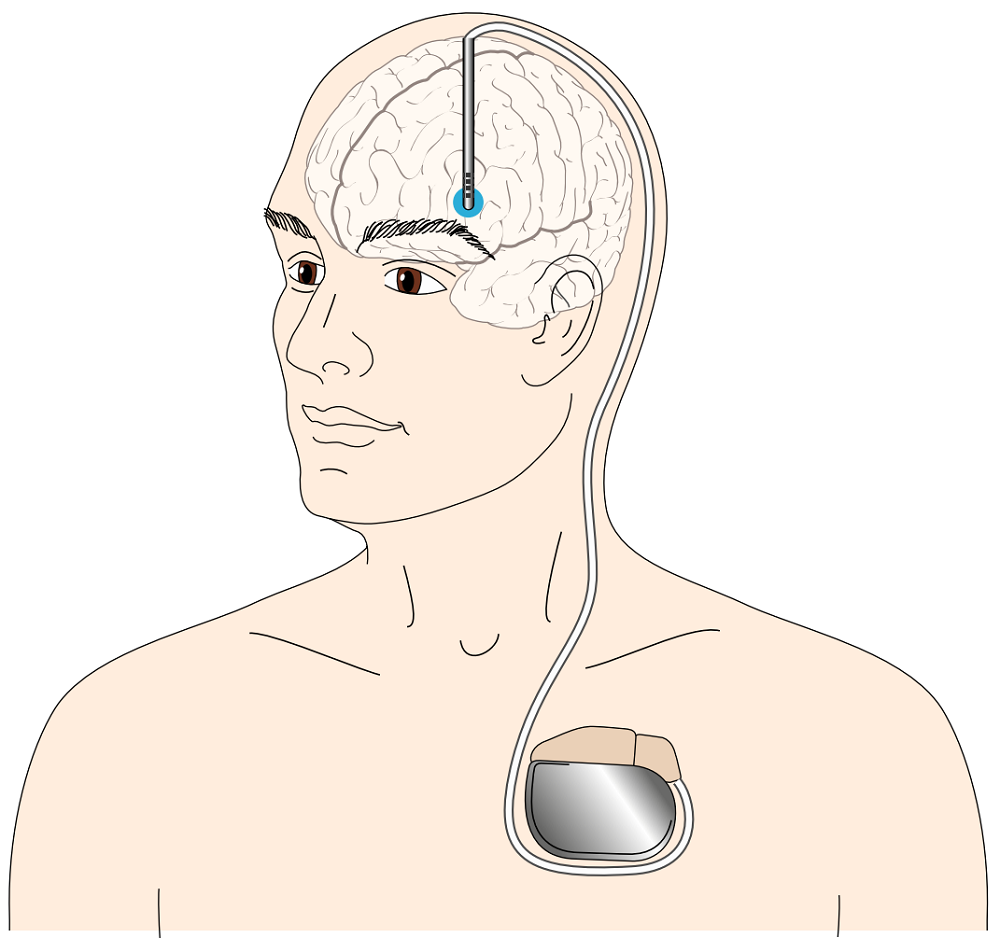
\includegraphics[width=\textwidth]{dbs00}
         \caption{
         الکترودها و تولید کننده های پالس به طور دائمی کاشته می شوند. 
         بسته به جانبی بودن علائم ، می توان الکترودها را در یک یا هر دو نیمکره مغز کاشت.
         الکترود (های) کاشته شده در مغز به مولد نبض کاشته شده در قفسه سینه متصل است.
         }
         \label{fig:dbs00}
     \end{subfigure}
    \
         \begin{subfigure}[t]{0.45\textwidth}
         \centering
         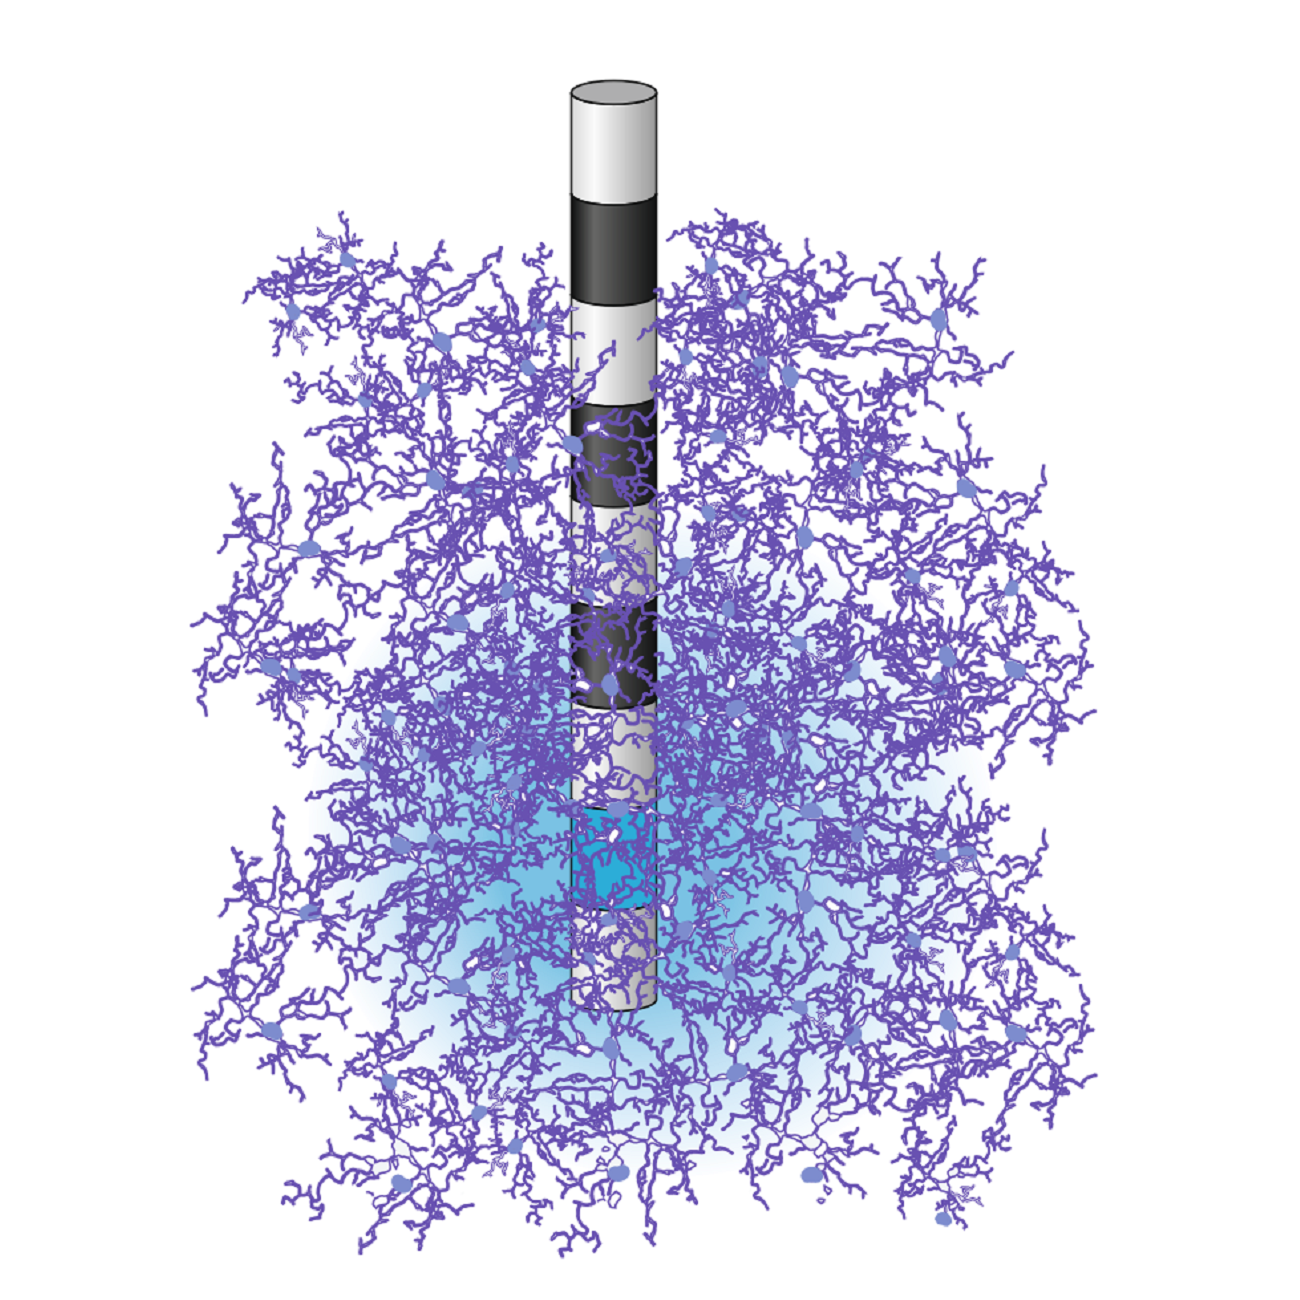
\includegraphics[width=\textwidth]{dbs01}
         \caption{  
         الکترودهای تحریک عمیق مغز سنتی از چهار نقطه تماس (استوانه های سیاه) تشکیل شده است ، که
         معمولاً از یکی از این نقاط تماس برای تحریک استفاده می شود.
         متداول ترین هدف جراحی برای درمان بیماری پارکینسون ، هسته زیر تالاموس است که تقریبا حاوی 250000 نورون  که با رنگ آبی به تصویر کشیده شده و در واقع بسیار متراکم تر از آنچه در اینجا نشان داده شده است.
         }
         \label{fig:dbs01}
     \end{subfigure}
     \caption{تحریک جریان مستقیم درون جمجمه ای از طریق الکترودهای متصل خارجی }
    \label{fig:dbs}
\end{figure}

%
%از مقاله ها:
%\\
برای بیش از 30 سال تحریک عمیق مغز برای هدف قرار دادن علائم تعدادی از اختلالات عصبی و به ویژه اختلالات حرکتی مانند بیماری پارکینسون و لرزش اساسی  استفاده شده است.

می‌دانیم که از دست دادن نورون های دوپامینرژیک در توده سیاه
\LTRfootnote{Substantia nigra}
 منجر به بیماری پارکینسون می‌شود، در حالی که تأثیر دقیق این امر بر دینامیک مغز کاملاً مشخص نیست، وجود فعالیت نوسانی باند بتا پاتولوژیک تصور می شود.    
با اینکه علت  لرزش اساسی هنوز ناشناخته است، با این حال، نوسانات پاتولوژیک در شبکه تالاموکورتیکال-مخچه با لرزش مرتبط است.

هر دو این اختلالات حرکتی با تحریک عمیق مغز درمان می شوند ، که لازمه این امر کاشت الکترود در مغز بیمار می‌باشد. در حالی که تحریک عمیق مغز منجر به بهبود علائم در بسیاری از بیماران می شود ، مکانیسم های اساسی این بهبود به روشنی درک نشده است
